\documentclass[letterpaper]{article}
\usepackage[submission]{aaai2027}
\usepackage[hyphens]{url}
\usepackage{graphicx}
\urlstyle{rm}
\def\UrlFont{\rm}
\usepackage{natbib}
\usepackage{caption}
\frenchspacing
\usepackage{booktabs}
\usepackage{amssymb}
\pdfinfo{/TemplateVersion (2027.1)}
\setcounter{secnumdepth}{2}
\title{Supplementary Material for ``Quantifying the Gaps: A Systematic Taxonomy of Bias and Imbalance in Multilingual AI Evaluation''}
\author{Anonymous submission}
\affiliations{Anonymous submission}
\begin{document}
\maketitle

\section{Classification Criteria and Annotation Protocol}
\label{sec:criteria}

Each of the 96 resources in the corpus (65 evaluation benchmarks, 2018--2025; 31 training datasets, 2005--2025) was annotated on all five taxonomy dimensions from its primary paper, dataset card, and repository. This section states the category definitions used for each dimension and the decision rules applied to mixed cases. Exactly two explicit decision rules govern mixed cases---the majority-composition rule for data origin (D1) and the designed-to-evaluate rule for resource tier (D2); no further tie-breaking heuristics were applied. Where a category boundary is not further specified below, the annotation follows the descriptive granularity of the resource's own primary sources.

\subsection{D1: Data Origin (\emph{native} $|$ \emph{translated})}
This dimension confronts the ``translationese'' problem by quantifying reliance on translated content versus natively sourced data.
\begin{description}
\item[Native.] The resource's content was originally authored or collected in the language(s) it covers, rather than produced by translation from a source language.
\item[Translated.] The resource's content was produced by machine or human translation from material originally created in another language.
\end{description}
\paragraph{Decision rule (mixed cases).} A resource that combines native and translated subsets is classified by its \emph{majority composition}: it is labeled \emph{native} if natively sourced content predominates, and \emph{translated} if translated content predominates.

\subsection{D2: Linguistic Resource Tier (\emph{high} $|$ \emph{medium} $|$ \emph{low})}
This dimension maps the divide between resource-rich and resource-poor languages, following established resource-level classifications \cite{joshi2020state}.
\begin{description}
\item[High.] The resource predominantly targets high-resource (resource-rich) languages under the established classification.
\item[Medium.] The resource predominantly targets medium-resource languages under the established classification.
\item[Low.] The resource centers low-resource (resource-poor) languages under the established classification.
\end{description}
\paragraph{Decision rule (mixed cases).} The tier assigned to a resource reflects the tier of the languages the benchmark is \emph{designed to evaluate}, not incidental coverage. A benchmark whose evaluative focus is high-resource languages is classified \emph{high} even if its language list incidentally includes lower-tier languages.

\subsection{D3: Task Class (13 classes)}
This dimension records which capability a benchmark actually measures, revealing the community's emphasis across tasks. Each benchmark is assigned to one of thirteen classes:
\emph{QA} (question answering);
\emph{syntax} (syntactic evaluation);
\emph{reasoning};
\emph{multimodal};
\emph{NLU} (natural language understanding);
\emph{summarization};
\emph{math} (mathematical problem solving);
\emph{RAG} (retrieval-augmented generation);
\emph{code} (code generation and understanding);
\emph{generation} (open-ended generation);
\emph{long-context};
\emph{embeddings};
and \emph{other}, a residual class for benchmarks whose evaluated task falls outside the twelve named classes. Assignment follows the task the resource itself evaluates, as stated in its primary paper and dataset card.

\subsection{D4: Cultural Specificity (\emph{universal} $|$ \emph{culturally anchored} $|$ \emph{region-specific})}
This dimension quantifies Anglocentric and Western-centric defaults by distinguishing benchmarks that are genuinely culture-independent from those that merely strip cultural context.
\begin{description}
\item[Universal.] The benchmark's content is culturally non-specific: it does not presuppose knowledge of a particular culture. As noted in the main text, this category encompasses both content that is genuinely culture-independent and content from which cultural context has been stripped; the annotation records non-specificity as presented by the resource, and the distinction between these two situations is itself one of the imbalances the taxonomy is designed to surface.
\item[Culturally anchored.] The benchmark's content is grounded in cultural knowledge or cultural context.
\item[Region-specific.] The benchmark's content is tied to a particular region.
\end{description}
No additional tie-breaking rule beyond these definitions was applied to this dimension; boundary cases were resolved from the resource's primary paper, dataset card, and repository at the level of description those sources provide.

\subsection{D5: Inference Paradigm}
This dimension captures two aspects of how a benchmark stresses model performance:
\begin{description}
\item[Nature of reasoning.] Whether the benchmark demands \emph{retrieval-style} inference or \emph{multi-hop} reasoning.
\item[Evaluation regime.] Whether evaluation proceeds by \emph{direct multilingual inference} (the model operates in the target language) or by \emph{Translate-Test} (inputs are translated into a pivot language before inference).
\end{description}
As with D3 and D4, no mixed-case decision rule applies to this dimension; annotations follow the paradigm reported by the resource's own evaluation setup.

\subsection{Corpus Screening}
Candidate resources were gathered by a targeted sweep of the ACM Digital Library, arXiv, the ACL Anthology, and Hugging Face Datasets (benchmarks published 2018--2025; training corpora 2005--2025). Each candidate passed a three-part screen:
\begin{enumerate}
\item \textbf{Public availability} of the dataset or a detailed benchmark description;
\item \textbf{Explicit multilingual or cross-lingual scope}; and
\item \textbf{Clear, reproducible evaluation results or metrics.}
\end{enumerate}
After screening and deduplication, 96 resources were retained: 65 evaluation benchmarks and 31 training datasets covering 139 unique languages. A small number of influential monolingual resources are retained only where they anchor an explicitly multilingual lineage---for instance, BLiMP's minimal-pair template as the design ancestor of syntactic benchmarks in Chinese, Turkish, Russian, Dutch, and 101-language form \cite{warstadt2020blimp}.

\subsection{How to Audit These Annotations}
The classification criteria stated here and the complete per-resource annotations are public, so every cell of the analysis can be traced from a resource's primary paper, dataset card, and repository to its five-dimensional label. We explicitly invite the community to audit these annotations: if a reader believes a resource is misclassified on any axis---for example, that a majority-translated benchmark is labeled native, or that a tier assignment mistakes incidental coverage for designed scope---we welcome corrections through the public release accompanying this paper. Because every aggregate statistic in the paper is computed directly from these annotations, any accepted correction propagates transparently to the reported figures, and we will maintain the released annotations as a living, correctable record of the multilingual evaluation landscape.

\section{Quantitative Companion Analyses}
\label{sec:quant}
This section derives the summary indices quoted in \S4 of the main paper and reports companion analyses. Every quantity below is computed solely from counts already printed in the main paper (Tables~1 and~2 and Figure~2); no unreleased data are required, so each derivation can be checked by hand.

\subsection{Coverage Inequality Across the World's Languages}
\label{sec:gini}
Let $x_\ell$ be the number of the 65 benchmarks covering language $\ell$, over the population of roughly 7{,}000 living languages \cite{joshi2020state}. Table~2 of the main paper fixes the twenty largest values exactly (sum 502, from English at 37 down to Greek at 13); its caption bounds each of the remaining 119 covered languages at $1 \le x_\ell \le 13$; and the remaining $\sim$6{,}861 languages have $x_\ell = 0$. The Gini coefficient of this distribution is bracketed by the two extreme tail allocations consistent with these constraints: setting all 119 tail values to 13 (the \emph{most equal} feasible allocation, which also maximizes total coverage) yields $G = 0.9823$, and setting all 119 to 1 (the least equal) yields $G = 0.9937$, with $G$ monotone between these extremes (verified numerically over random feasible tails). Benchmark coverage across living languages therefore has a Gini coefficient between 0.982 and 0.994 \emph{regardless} of the unobserved tail values. Restricted to only the 139 covered languages, the same construction is uninformative ($G \in [0.106, 0.681]$); the all-languages population---the population over which the main paper's equity claims are made---is the appropriate frame. Figure~\ref{fig:supp-decay} shows the distribution itself: a twenty-language head, a bounded tail, and $6{,}800+$ languages at zero. Figure~\ref{fig:supp-lorenz} renders the same result as a Lorenz curve: the two feasible extremes bracket every possible true curve, and both hug zero across 98\% of the language axis before rising almost vertically---coverage concentration near the theoretical maximum.

\begin{figure}[t]
\centering
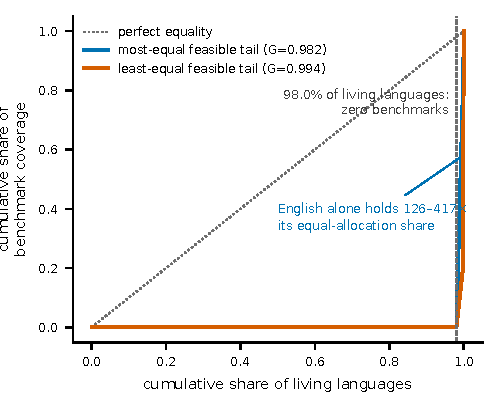
\includegraphics[width=\columnwidth]{supp_fig_lorenz.pdf}
\caption{Lorenz curves of benchmark coverage over $\sim$7{,}000 living languages under the two extreme feasible tail allocations. The true curve lies between them; the Gini coefficient is $G \in [0.982, 0.994]$ regardless of the unobserved tail values. The dashed vertical line marks the 98.0\% of living languages covered by no benchmark in the corpus.}
\label{fig:supp-lorenz}
\end{figure}

\begin{figure}[t]
\centering
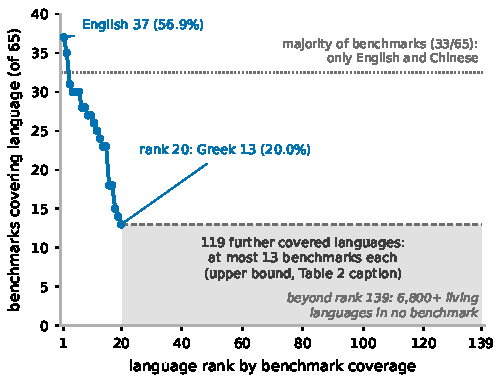
\includegraphics[width=\columnwidth]{supp_fig_decay.pdf}
\caption{Benchmark coverage by language rank, drawn entirely from Table~2 of the main paper and its caption. The twenty verified head values account for 502 language--benchmark inclusions; the shaded band is the caption's upper bound of 13 for each of the 119 remaining covered languages. Only English and Chinese appear in a majority of the 65 benchmarks, and coverage falls 65\% (37$\to$13) within the head alone.}
\label{fig:supp-decay}
\end{figure}

\subsection{Concentration Indices for the Task, Tier, and Cultural Axes}
\label{sec:diversity}
Effective-number diversity indices summarize how evenly the 65 benchmarks spread across nominal categories. Over the thirteen task classes (QA~20, syntax~12, reasoning~6, multimodal~6, NLU~5, summarization~4, math~3, RAG~2, code~2, generation~2, other~1, long-context~1, embeddings~1), the Herfindahl--Hirschman concentration is $\sum_i p_i^2 = 0.161$, an inverse-Simpson effective number of $6.2$ task classes; the Shannon entropy is 2.14 nats (perplexity 8.5; evenness 0.83 of the $\ln 13$ maximum). The field nominally spans thirteen capabilities but effectively measures about six. The resource-tier distribution (46/15/4) concentrates further: HHI $= 0.558$, an effective 1.8 of 3 tiers; the cultural axis (36/17/12) yields an effective 2.4 of 3 categories. These indices make the main paper's task monoculture (\S4.3) and tier skew (\S4.1) reportable as single numbers that audits of other evaluation ecosystems can reproduce for comparison.

A cell-level corollary follows from the marginals alone: because only 4 of 65 benchmarks center low-resource languages, the low-resource row of the tier~$\times$~task matrix can contain at most 4 nonzero cells---at least 9 of its 13 cells are exactly empty, whichever tasks those four benchmarks cover. The emptiness of most low-resource capability cells named in the main paper's roadmap is thus guaranteed by arithmetic, not merely observed; identifying \emph{which} nine requires the released annotations.

\subsection{Are the Benchmark and Dataset Distributions the Same? Homogeneity Tests}
\label{sec:homogeneity}
\S4.5 of the main paper reads evaluation gaps and data gaps as ``the same gap seen from two directions.'' Chi-square homogeneity tests on Table~1's marginals quantify the mirroring between the 65 benchmarks and 31 training datasets (Table~\ref{tab:homogeneity}): on no shared axis do the two populations differ detectably, and every effect size is small (largest Cram\'er's $V = 0.15$, on cultural grounding, driven by the datasets' higher universal share). Two caveats apply: non-rejection at $n = 96$ bounds similarity rather than proving equivalence---the effect sizes, not the $p$-values, carry the claim---and the low-tier cells have small expected counts (minimum 1.94), so the tier test is approximate. Figure~\ref{fig:supp-dumbbell} shows the eight category-level share comparisons directly.

\begin{table}[t]
\centering
\small
\begin{tabular}{@{}lrrrr@{}}
\toprule
Axis & $\chi^2$ & df & $p$ & Cram\'er's $V$ \\
\midrule
Origin (native/translated) & 0.00 & 1 & 0.97 & 0.00 \\
Tier (high/medium/low) & 0.62 & 2 & 0.73 & 0.08 \\
Cultural (univ./anch./region) & 2.29 & 2 & 0.32 & 0.15 \\
\bottomrule
\end{tabular}
\caption{Homogeneity of the 65 benchmarks vs.\ the 31 training datasets on the three shared axes (counts from Table~1 of the main paper). Fisher's exact test on the origin axis gives $p = 1.00$.}
\label{tab:homogeneity}
\end{table}

\begin{figure}[t]
\centering
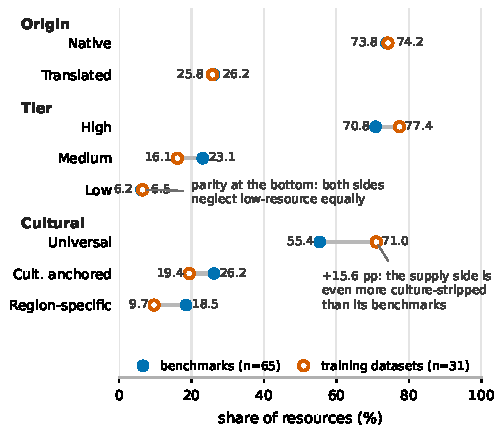
\includegraphics[width=\columnwidth]{supp_fig_dumbbell.pdf}
\caption{Benchmark share (filled) vs.\ training-dataset share (open) for every category on the three shared axes---all sixteen values from Table~1 of the main paper. The supply side is more culture-stripped (universal $+15.6$ percentage points) and more high-tier-concentrated ($+6.6$\,pp) than the benchmarks it feeds, while the two sides neglect low-resource languages in near-identical proportion (6.2\% vs.\ 6.5\%).}
\label{fig:supp-dumbbell}
\end{figure}

\subsection{Temporal Production: The Surge Is Evaluation-Only}
\label{sec:temporal}
Crossing the two per-year series in Figure~2 of the main paper yields the production comparison quoted in its caption. Through 2023, benchmark and training-dataset creation ran near parity: 27 benchmarks vs.\ 23 datasets (1.2:1). In 2024--2025 the ratio flipped to 38 vs.\ 8 (4.8:1); the association between era and resource type is significant (Fisher's exact test on the $2\times2$ table of era by resource type: odds ratio 4.05, $p = 0.004$). Cumulatively, 74.2\% of the training corpora but only 41.5\% of the benchmarks existed by the end of 2023 (benchmark milestones: 20.0\% by 2021, 41.5\% by 2023, 80.0\% by 2024). Descriptively, data supply has historically led evaluation by about a year: dataset production in year $t$ correlates with benchmark production in year $t{+}1$ at Pearson $r = 0.77$ over the seven overlapping year-pairs, versus $r = 0.47$ contemporaneously and $r = -0.30$ for the reverse lag. With so few years and a right-truncated 2025, we report these correlations as descriptive only; the era-level flip, not the lag, is the robust finding. Read with \S4.5 of the main paper, the implication is directional: the field is currently certifying capabilities faster than it is supplying the data to build them, and today's 6.5\% low-resource dataset share is positioned to cap the low-resource benchmark share for years.

\subsection{What Would Count-Parity Take?}
\label{sec:parity}
The roughly 1.2 billion speakers of effectively unmeasured languages (\S1 of the main paper) are about 15\% of the world's population ($1.2/8.1 \approx 14.8\%$). Lifting the low-resource benchmark share from its current 6.2\% (4 of 65) to speaker-share parity would require only seven additional low-resource-centered benchmarks ($11/72 = 15.3\%$); the dataset side would require three ($5/34 = 14.7\%$). Against the field's 2024--2025 production rate of 19 benchmarks per year (38 in two years; Figure~2 of the main paper), seven benchmarks is about 4.4 months of output. Count-parity is a redirection of one research season, not a decade-scale program; parity of \emph{quality} additionally requires the natively sourced, culturally grounded construction that R1 and R2 of the main paper specify.

\section{Per-Resource Structured Summaries: Training Datasets}

This section provides condensed, structured summaries of the 31 training datasets analyzed in the main paper, organized by primary purpose (pre-training corpora, translation/alignment corpora, and instruction fine-tuning datasets). Each entry records key statistics on size, language coverage, construction method, and intended purpose.

\subsection{Pre-training Corpora}

\paragraph{FineWeb (2024)} FineWeb is a 15-trillion-token English dataset derived from 96 Common Crawl snapshots and designed to train high-performing LLMs \citep{penedo2024finewebdatasetsdecantingweb}. Its creators address the opacity of pre-training data curation by documenting and ablating deduplication and filtering strategies, and additionally release FineWeb-Edu, a 1.3-trillion-token educational subset that improves knowledge and reasoning benchmark performance. The data-curation codebase and all ablation models are publicly released.

\paragraph{FineWeb-2 (2025)} FineWeb-2 is a model-based filtering framework for multilingual pre-training data that uses Transformer- and FastText-based classifiers to select diverse, knowledge-rich samples \citep{messmer2025enhancingmultilingualllmpretraining}. Ablations across language families, scripts, and resource levels show that a 1B-parameter Llama model can match the full-data MMLU score using as little as 15\% of the tokens. The framework is extended to 20 languages and the refined datasets are publicly released.

\paragraph{HPLT (2024--2025)} The HPLT (High Performance Language Technologies) resources are massive multilingual corpora extracted from CommonCrawl and the Internet Archive \citep{degibert2024newmassivemultilingualdataset,burchell2025expandedmassivemultilingualdataset}. Version~1 comprises roughly 5.6 trillion monolingual tokens in 75 languages plus 96 million English-centric parallel sentence pairs across 18 language pairs; version~2 expands this to 8 trillion tokens in 193 languages and 380 million parallel pairs in 51 languages. They are among the largest open text corpora released and are shown useful for training language and machine-translation models.

\paragraph{C4 (2020)} The Colossal Clean Crawled Corpus (C4) was introduced alongside a unified text-to-text transfer-learning framework that recasts all text problems in a text-to-text format \citep{raffel2023exploringlimitstransferlearning}. C4 was used to train the T5 model, enabling a systematic study of pre-training objectives, architectures, and datasets and achieving state-of-the-art results across summarization, question answering, and classification. The dataset, models, and code were released and have become foundational for subsequent work.

\paragraph{CulturaX (2023)} CulturaX is a 6.3-trillion-token multilingual dataset covering 167 languages, built to address transparency and quality gaps in LLM training data \citep{nguyen2023culturaxcleanedenormousmultilingual}. It is produced through a multi-stage pipeline of language identification, URL-based filtering, metric-based cleaning, document refinement, and deduplication. The dataset is fully released on HuggingFace to support research on hallucination, bias, and replication.

\paragraph{MADLAD-400 (2023)} MADLAD-400 is a manually audited, general-domain, 3-trillion-token monolingual dataset based on CommonCrawl and covering 419 languages \citep{kudugunta2023madlad400multilingualdocumentlevellarge}. The authors emphasize the role of self-auditing in surfacing dataset limitations. Using this and other data they train a 10.7B-parameter multilingual MT model spanning over 450 languages that is competitive with much larger models, plus an 8B language model; baseline models are released.

\paragraph{RedPajama (2024)} RedPajama is a large-scale open dataset addressing the lack of transparency in proprietary data curation \citep{weber2024redpajamaopendatasettraining}. It comprises RedPajama-V1, an open reproduction of the LLaMA training data, and RedPajama-V2, a web-only corpus of over 100 trillion tokens accompanied by quality signals and metadata. Ablations with models up to 1.6B parameters show the quality signals enable high-quality subset curation, and the data has been used to train production models such as Snowflake Arctic and Salesforce XGen.

\paragraph{OpenWebText (2019)} OpenWebText is an open-source replication of OpenAI's WebText corpus used to train GPT-2 \citep{Gokaslan2019OpenWeb}. URLs were extracted from the Reddit submissions dataset, deduplicated, and filtered to HTML content; pages were extracted with the newspaper package, non-English text removed via FastText, near-duplicates removed with LSH over 5-gram sets (similarity $>0.5$), and documents under 128 tokens dropped. The final corpus contains 38GB of text across 8,013,769 documents and is released under CC0.

\paragraph{OSCAR (2020)} OSCAR is a large multilingual corpus extracted from Common Crawl, studied here for building monolingual contextualized embeddings for mid-resource languages \citep{ortiz-suarez-etal-2020-monolingual}. Monolingual ELMo embeddings trained on OSCAR for five languages significantly outperform Wikipedia-trained embeddings on POS tagging and parsing, and set a new state of the art surpassing multilingual BERT. The work underscores the value of web-scale monolingual data for mid-resource languages.

\paragraph{Common Corpus (2025)} Common Corpus is described as the largest open dataset for LLM pre-training, with approximately two trillion tokens \citep{langlais2025commoncorpuslargestcollection}. It is designed to comply with AI legislation and data-security regulations by including only uncopyrighted or permissibly licensed content, spans major European through low-resource languages, and includes substantial code. The authors detail their assembly, filtering, and curation process; the corpus is already in industrial use and intended as open-science infrastructure.

\paragraph{ROOTS (2023)} The Responsible Open-science Open-collaboration Text Sources (ROOTS) corpus is a 1.6TB dataset spanning 59 languages, created within the BigScience workshop \citep{laurençon2023bigsciencerootscorpus16tb}. It was used to train the 176-billion-parameter BLOOM language model. A large subset and the processing tools are released to support monolingual and multilingual modeling research.

\paragraph{IndicNLPSuite / IndicCorp (2020)} This series provides NLU resources for Indian languages \citep{kakwani-etal-2020-indicnlpsuite,doddapaneni2023leavingindiclanguagebehind}. IndicNLPSuite introduced monolingual corpora for 11 Indian languages (8.8 billion tokens), FastText embeddings, ALBERT language models, and the IndicGLUE benchmark; the follow-up adds IndicCorp (20.9 billion tokens across 24 languages), the IndicXTREME benchmark of nine NLU tasks across 20 languages, and IndicBERT~v2, which improves 2 points over strong baselines. All resources are publicly available.

\paragraph{IndicLLMSuite (2024)} IndicLLMSuite is a resource suite for building LLMs across 22 Indian languages, comprising a 251-billion-token pre-training corpus and a 74.8-million-pair instruction-tuning dataset \citep{Khan_2024}. An open-source pipeline curates data from websites, PDFs, and videos, while instruction data combines existing Indic datasets, translated/transliterated English data, and synthetic conversations from LLaMa2 and Mixtral; a toxicity-alignment dataset of toxic prompts with non-toxic responses is also included. It is released under permissive licenses.

\paragraph{Norwegian Colossal Corpus (2022)} The Norwegian Colossal Corpus (NCC) is a 49GB corpus of clean Norwegian text with over 7 billion words, created to address the shortage of Norwegian training data \citep{kummervold-etal-2022-norwegian}. It draws on books, newspapers, government documents, and public reports and covers both Bokm{\aa}l and Nynorsk, with per-document metadata enabling sub-corpus creation. The corpus is openly available.

\paragraph{SEA-LION (2025)} SEA-LION is a family of models targeting the under-representation of Southeast Asian languages, including Llama-SEA-LION-v3-8B-IT and Gemma-SEA-LION-v3-9B-IT supporting 11 SEA languages \citep{ng2025sealionsoutheastasianlanguages}. Training combines large-scale multilingual continued pre-training with multi-stage instruction fine-tuning, alignment, and model merging, achieving state-of-the-art results on SEA multilingual benchmarks. The work is associated with the 120-billion-token SEA-PILE dataset and is open-sourced.

\paragraph{Nepali Transformer Models (2025)} This work presents pre-trained transformer models for Nepali, a low-resource language with 32 million speakers \citep{thapa2025developmentpretrainedtransformerbasedmodels}. A 27.5GB corpus, 2.4 times larger than prior corpora, was scraped from 99 news websites, preprocessed with deduplication, language filtering, and Unicode normalization, and used to train BERT (110M), RoBERTa (125M), and GPT-2 (124M). On the Nep-gLUE benchmark the RoBERTa model reaches 95.60 (2 points over the prior best), and the instruction-tuned GPT-2 achieves ROUGE-L of 17.76 on summarization.

\paragraph{UCCIX (2024)} UCCIX is the first large-scale open-source Irish language model, built on Llama~2-13B via an efficient continued pre-training framework for extremely low-resource settings \citep{tran2024uccixirishexcellencelargelanguage}. From a 1.8-billion-character Irish corpus, staged adaptation beginning with parallel English--Irish data and a 10,000-token Irish tokenizer extension precede supervised instruction fine-tuning; the resulting UCCIX-Instruct surpasses much larger models such as Llama~2-70B and BLOOM-7B by up to 12\% on key tasks. The authors also release the IrishQA benchmark and an Irish-translated MT-bench, while noting partial catastrophic forgetting of English.

\paragraph{SERENGETI (2023)} SERENGETI is a massively multilingual language model covering 517 African languages and varieties, greatly expanding beyond the roughly 31 African languages in prior models \citep{adebara2023serengetimassivelymultilinguallanguage}. Across eight NLU tasks over 20 datasets it outperforms competing models on 11 datasets with an average F1 of 82.27, and the paper analyzes the effect of language genealogy and similarity on zero-shot performance. The models are publicly available for research.

\paragraph{African T5 Corpus (2023)} This work introduces a higher-quality multilingual pre-training corpus for 16 African languages, produced by auditing and cleaning web-crawled data from sources such as mC4 \citep{oladipo-etal-2023-better}. A T5-based model trained on the cleaned data outperforms existing pre-trained models on four downstream tasks and is more than twice as effective as multilingual T5 on cross-lingual QA. All code, data, and models are publicly released, underscoring the role of data quality in low-resource pre-training.

\subsection{Translation/Alignment Corpora}

\paragraph{CCMatrix (2020)} CCMatrix is a massive parallel corpus built by applying margin-based bitext mining to billions of Common Crawl sentences \citep{schwenk2020ccmatrixminingbillionshighquality}. A unified approach across 38 languages mined 4.5 billion parallel sentences, 661 million aligned with English. NMT systems trained solely on the mined data set new state-of-the-art WMT'19 results for English--German, English--Russian, and English--Chinese, demonstrating the value of large-scale web bitext mining.

\paragraph{CCAligned (2020)} CCAligned is a dataset of cross-lingual web-document pairs created by exploiting URL signals across 68 Common Crawl snapshots \citep{el-kishky-etal-2020-ccaligned}. It contains over 392 million URL pairs across 8,144 language pairs (137 involving English) with an average precision of 94.5\%, plus baseline methods for content-based alignment using cross-lingual representations. Parallel sentences mined from it train strong MT models, making it valuable for low- and medium-resource cross-lingual NLP.

\paragraph{ParaCrawl (2020)} ParaCrawl is an effort to build the largest publicly available parallel corpora by crawling the web, releasing open-source software and methods for web-scale parallel-data acquisition \citep{banon-etal-2020-paracrawl}. The authors empirically compare sentence-alignment and filtering methods, release benchmark datasets for those tasks, and evaluate the corpora's usefulness for MT. ParaCrawl has become a key large-scale parallel-data resource for many languages.

\paragraph{WikiMatrix (2021)} WikiMatrix is a parallel corpus mined from Wikipedia articles in 96 languages using multilingual sentence embeddings \citep{schwenk-etal-2021-wikimatrix}. It contains 135 million parallel sentences across 1,620 language pairs, with only 34 million aligned to English, yielding many direct non-English alignments. NMT systems trained for 1,886 language pairs and evaluated on the TED corpus achieve strong BLEU, making it especially useful for distant language pairs without English pivoting.

\paragraph{Europarl (2005)} Europarl is a parallel corpus of 11 languages drawn from European Parliament proceedings and one of the first large-scale, publicly available parallel corpora \citep{koehn-2005-europarl}. The paper describes its acquisition and application as SMT training data, with systems trained for 110 language pairs. Europarl has been foundational for the development and evaluation of machine-translation systems.

\paragraph{OpenSubtitles2018 (2018)} This work improves sentence alignments in the large, noisy OpenSubtitles parallel corpus derived from movie and TV subtitles \citep{lison-etal-2018-opensubtitles2018}. A statistical rescoring method addresses the alignment challenges of such noisy data. The widely used corpus provides parallel data for many language pairs, and the improved alignments enhance its value for training and evaluating cross-lingual models.

\paragraph{Tatoeba Translation Challenge (2020)} The Tatoeba Translation Challenge is a machine-translation benchmark providing training and test data for thousands of language pairs across over 500 languages \citep{tiedemann-2020-tatoeba}. It offers realistic low-resource scenarios, systematic language and script annotation, and data splits extending existing benchmark coverage. The release also includes a growing set of pre-trained baseline models to spur open translation tools.

\subsection{Instruction Fine-tuning Datasets}

\paragraph{Aya Dataset (2024)} The Aya Dataset is a large-scale, human-curated instruction-following dataset created to close the language gap in instruction-tuning resources \citep{singh2024aya}. Fluent speakers worldwide collected natural instruction--completion instances in 65 languages, complemented by the Aya Collection of 513 million templated and translated instances across 114 languages. The initiative also produced the Aya Annotation Platform and Aya Evaluation Suite, serving as a model for participatory research.

\paragraph{Bactrian-X (2023)} Bactrian-X is a multilingual parallel dataset of 3.4 million instruction--response pairs across 52 languages, addressing the scarcity of high-quality multilingual instruction-tuning data \citep{li2023bactrianxmultilingualreplicableinstructionfollowing}. Using it, the authors train lightweight LoRA adapters that plug into LLMs per language or language group and outperform both vanilla and existing instruction-tuned models across multilingual settings. Code and models are publicly available.

\paragraph{xP3 (2023)} xP3 is a composite of supervised datasets in 46 languages with English and machine-translated prompts, introduced to study crosslingual generalization via multitask prompted finetuning (MTF) \citep{muennighoff2023crosslingualgeneralizationmultitaskfinetuning}. Applying MTF to BLOOM and mT5 produces the BLOOMZ and mT0 variants, showing that English-task finetuning generalizes to non-English languages and that multilingual tasks with English prompts improve performance further. The code, datasets, and models are released publicly.

\section{Per-Resource Structured Summaries: Evaluation Benchmarks}

This supplement provides condensed structured summaries of the evaluation benchmarks surveyed in the main paper, grouped by task class. Each entry notes scope, language coverage, construction methodology, and headline results, with original citations preserved.

\subsection{Question Answering (QA)}

\paragraph{XQuAD (2020)} \citep{Artetxe_2020} introduce XQuAD alongside MONOTRANS, a method that transfers a monolingual masked language model to new languages by learning new embedding matrices while freezing the transformer body. XQuAD contains 240 context paragraphs and 1,190 question--answer pairs from SQuAD v1.1, professionally translated into ten languages (Spanish, German, Greek, Russian, Turkish, Arabic, Vietnamese, Thai, Chinese, Hindi). Results show MONOTRANS is competitive with jointly trained multilingual models, challenging the need for shared vocabularies or joint multilingual training for cross-lingual generalization.

\paragraph{MLQA (2019)} \citep{lewis2019mlqa} present a multi-way aligned benchmark for cross-lingual extractive QA across seven languages, with over 12,000 instances in English and over 5,000 in each of Arabic, German, Spanish, Hindi, Vietnamese, and Simplified Chinese. Construction combined automatic identification of parallel Wikipedia sentences, crowd-sourced English QA pairs, and professional translation with target-language answer annotation, yielding instances parallel across four languages on average. Evaluations of state-of-the-art cross-lingual models and machine-translation baselines show transfer performance significantly behind English performance.

\paragraph{BELEBELE (2023)} \citep{bandarkar2023belebele} present a parallel machine reading comprehension benchmark of 900 multiple-choice questions across 122 language variants, each based on a FLORES-200 passage and translated by human experts. Questions were curated with strong negative answers to punish pattern-matching heuristics while remaining solvable by humans with near-perfect accuracy. Results show large English-centric LLMs exhibit surprising cross-lingual generalization, while smaller masked language models pretrained on balanced multilingual data understand far more languages.

\paragraph{Indic-QA Benchmark (2024)} \citep{singh2024indic} construct the largest publicly available context-grounded QA dataset for 11 major Indian languages, compiling existing datasets, translating major English QA benchmarks, and generating a manually verified synthetic dataset covering extractive and abstractive QA. Evaluations of multilingual LLMs reveal weak performance, especially in low-resource languages, attributed to English bias in training. The Translate-Test paradigm (translating inputs to English and back) significantly outperforms direct multilingual inference, particularly in low-resource settings.

\paragraph{ECLEKTIC (2025)} \citep{goldman2025eclekticnovelchallengeset} present a closed-book QA benchmark for cross-lingual knowledge transfer, targeting Wikipedia facts available in only one of 12 languages and translating them into all others, with 4,608 human-verified QA pairs. Evaluations of 8 LLMs show the best model (Gemini 2.0 Pro) achieves only 41.6\% overall success and 65\% transfer score, revealing that models recall facts in the source language but fail to reproduce them in target languages. Shared script eases transfer, while relative transfer ability saturates around 14B parameters.

\paragraph{TeQuAD (2022)} \citep{vemula-etal-2022-tequad} present a large-scale Telugu QA dataset of 82,000 parallel English--Telugu triples created by translating SQuAD v1.1, using heuristics (cosine similarity, fuzzy matching, position indicators) and a supervised Dual BERT span-extraction model to map answer spans, with manual corrections for fluency and adequacy. Evaluation with mBERT under monolingual and cross-lingual setups achieves up to 83\% F1 and 61\% Exact Match, significantly outperforming TyDiQA and zero-shot baselines.

\paragraph{KenSwQuAD (2023)} \citep{10.1145/3578553} present a Swahili QA dataset of 1,445 story texts with 7,526 QA pairs, created from the Kencorpus Swahili corpus via purposive sampling and annotated by trained native speakers. Quality control on 12.5\% of the data showed 53.9\% exact matches and 37.9\% contextually similar answers. Proof-of-concept experiments achieved 80\% Precision@1 with a SPARQL-queried semantic network and 59.4\% F1 with fine-tuned XLM-RoBERTa, establishing a benchmark for Swahili QA adaptable to other low-resource languages.

\paragraph{FQuAD2.0 (2022)} \citep{heinrich-etal-2022-fquad2} extend FQuAD1.1 with over 17,000 adversarial unanswerable French questions (nearly 80,000 total), categorized into antonym negations, entity swaps, ambiguity, out-of-context, and semantic similarity. CamemBERT-LARGE achieves 83\% F1 and 82.3\% NoAnsF1, and the benchmark proves more challenging than English SQuAD2.0 under similar conditions; English-trained XLM-RoBERTa performs reasonably zero-shot in French but is outperformed by French monolingual models.

\paragraph{Global-MMLU (2024)} \citep{singh2024global} release an improved multilingual MMLU spanning 42 languages with translations verified by professional and community annotators, split into Culturally-Sensitive (CS) and Culturally-Agnostic (CA) subsets. Analysis shows 28\% of MMLU questions require culturally sensitive knowledge and 84.9\% of its geographic questions focus on North America or Europe. Re-evaluating 14 models demonstrates that rankings change significantly depending on the subset, with far greater variability on CS data.

\paragraph{IndicMMLU-Pro (2025)} \citep{sankalp2025indicmmlu} translate MMLU-Pro into nine Indic languages (Hindi, Bengali, Gujarati, Marathi, Kannada, Punjabi, Tamil, Telugu, Urdu) using IndicTrans2, with quality assurance via back-translation, automated metrics (chrF++, BLEU, METEOR, TER, SacreBLEU), and manual proofreading of 9,000 sentence pairs by 13 expert reviewers. Baseline results show GPT-4o consistently outperforms all other models across the nine languages, with accuracy from 38.46\% to 44.80\%.

\paragraph{MMLU-ProX (2025)} \citep{xuan2025mmlu} extend MMLU-Pro to 29 typologically diverse languages with 11,829 parallel questions per language (plus a 658-question lite version), using a semi-automated framework of LLM translation, self-reflection, LLM verification, and review by over 30 human experts. Evaluation of 36 LLMs reveals declines of up to 24.3\% on low-resource languages relative to high-resource ones, with reasoning-enhanced models showing better multilingual generalization.

\paragraph{ArabicMMLU (2024)} \citep{koto2024arabicmmlu} present the first massive multitask benchmark for Arabic, with 14,575 multiple-choice questions across 40 tasks sourced from school and professional exams in eight countries, curated with native speakers so that over 50\% of questions cover Arabic-specific topics. Evaluating 35 models, the top Arabic-centric model Jais-chat reaches only 62.3\% accuracy and GPT-4 performs best at 72.5\%, lower than its translated-MMLU score, indicating a more challenging and authentic benchmark.

\paragraph{CMMLU (2023)} \citep{li2023cmmlu} manually construct 11,528 multiple-choice questions across 67 subjects grounded in Chinese linguistic and cultural context, collected from non-public sources and mock exams to minimize contamination. Most of the 20+ evaluated LLMs fail to reach 60\% accuracy, with GPT-4 leading at 71\%; the best Chinese-oriented model, Baichuan2-13B, outperforms much larger multilingual models such as LLaMA2-70B.

\paragraph{TurkishMMLU (2024)} \citep{yuksel2024turkishmmlu} present the first multitask multiple-choice benchmark for Turkish, with over 10,000 questions covering nine Turkish high-school curriculum subjects, curated from an expert-written platform of the Turkish Ministry of Education and annotated with a difficulty-indicating correctness ratio from real student performance. Evaluation of over 20 LLMs shows closed-source models significantly ahead: GPT-4o achieves the top score of 83.1\% versus 67.3\% for the best open-source model (Llama-3 70B-IT).

\paragraph{KMMLU (2024)} \citep{son2024kmmlu} build a Korean benchmark of 35,030 expert-level multiple-choice questions across 45 subjects sourced entirely from original Korean exams, with one-fifth of questions requiring specific cultural, regional, or legal knowledge. Across 24 LLMs the top performer, GPT-4, scores just 59.95\%, far below the typical 80\% exam pass mark, while the Korean-specific HyperCLOVA X outperforms GPT-4 on localized subjects such as Korean History.

\paragraph{PAWS-X (2019)} \citep{yang2019paws} present a cross-lingual adversarial paraphrase identification dataset of 23,659 human-translated pairs in French, Spanish, German, Chinese, Japanese, and Korean, extending challenging PAWS examples with high lexical overlap but potentially different meanings. Multilingual BERT fine-tuned on English PAWS plus machine-translated data performs best, with an average accuracy gain of 23\% over the next best model across the six non-English languages.

\paragraph{m-ArenaHard / Aya Expanse (2024)} \citep{dang2024aya} introduce the Aya Expanse 8B and 32B open-weight multilingual models, built with multilingual data arbitrage, iterative preference training, and model merging, and release m-ArenaHard, a multilingual evaluation dataset translated from Arena-Hard-Auto into 23 languages. Aya Expanse models outperform leading open-weight competitors in their parameter classes, with the 32B model surpassing Llama 3.1 70B with a 54.0\% win-rate on m-ArenaHard.

\paragraph{MultiLoKo (2025)} \citep{hupkes2025multiloko} present a benchmark of locally relevant knowledge across 31 languages, with 500 locally sourced questions per language plus human- and machine-authored translations to and from English, a public development set, a blind test set, and metrics for parity, knowledge transfer, and translation effects. None of 11 evaluated multilingual LLMs perform well: the top model achieves only a 34.4\% average score, with large cross-language gaps and a pronounced ``mother tongue effect'' indicating suboptimal transfer.

\paragraph{BenchMAX (2025)} \citep{huang2025benchmaxcomprehensivemultilingualevaluation} introduce a multilingual suite covering 17 languages from 11 families and six advanced capabilities: instruction following, math/science reasoning, code generation, long-context understanding, tool use, and translation, built by machine translation from English post-edited by three native annotators with GPT-4o-mini as LLM-judge. Experiments across LLaMA-3.1, Qwen2.5, Gemma2, Aya-Expanse, InternLM2.5, DeepSeek-V3, and GPT-4o-mini show that scaling improves averages but English--non-English gaps persist, especially for low-resource languages such as Telugu, Swahili, and Bengali.

\paragraph{P-MMEval (2025)} \citep{zhang2025pmmevalparallelmultilingualmultitask} unify eight benchmarks (XNLI, MHELLASWAG, FLORES-200, MGSM, MMMLU, MLOGIQA, HUMANEVAL-XL, MIFEVAL) into a parallel multilingual multitask suite covering 10 languages from 7 families with expert-reviewed translations, and introduce the Cross-lingual Accuracy Consistency Ratio (CACR) to quantify transfer. Evaluations of open- and closed-source models show larger models improve multilingual transfer, with code and math transferring best and logical reasoning worst, and Thai/Japanese lagging behind Spanish/Portuguese.

\subsection{Syntax}

\paragraph{MultiBLiMP 1.0 (2025)} \citep{jumelet2025multiblimp10massivelymultilingual} present a massively multilingual benchmark of over 128,000 linguistic minimal pairs across 101 languages, focusing on subject--verb and subject--participle agreement, generated via an automated pipeline over Universal Dependencies and UniMorph. Evaluations of 42 LLMs show linguistic competence correlates with model size and language frequency in training data, instruction tuning can reduce multilingual fluency, and monolingual models with sufficient data outperform larger multilingual LLMs on several languages.

\paragraph{BLiMP (2020)} \citep{warstadt2023blimpbenchmarklinguisticminimal} present a benchmark of 67 paradigms covering 12 major English grammatical phenomena, generated from linguist-crafted templates as controlled minimal pairs and validated with human judgments (96.4\% agreement). Comparing n-gram, LSTM, Transformer-XL, and GPT-2 probabilities without supervision, models perform well on morphological agreement but struggle with NPI licensing, argument structure, and syntactic islands, underperforming humans; training data volume matters more than model size.

\paragraph{ZhoBLiMP (2024)} \citep{liu2024zhoblimpsystematicassessmentlanguage} present a Chinese minimal-pairs benchmark of 35,000 pairs across 118 paradigms covering 15 linguistic phenomena, generated from linguist-crafted templates with a curated vocabulary. Evaluating 20 models trained from scratch (10M--3B tokens) and 14 off-the-shelf LLMs, models with roughly 410M parameters trained on 1B tokens learn much of Chinese grammar, though anaphora, ellipsis, and quantifiers remain challenging, with U-shaped learning curves mirroring child language acquisition.

\paragraph{TurBLiMP (2025)} \citep{basar2025turblimp} present the first comprehensive Turkish minimal-pairs benchmark: 16,000 pairs across 16 grammatical phenomena plus 2,000 experimental pairs on word order and subordination, built via manual crafting, semi-automatic augmentation with BERTurk, and automated lexical replacement, validated by 30 native speakers. Across 13 models, larger models generally do better but monolingual Turkish models often surpass larger multilingual ones, with ellipsis, island effects, and relative clauses remaining difficult; BERTurk correlates best with human judgments.

\paragraph{BLiMP-NL (2025)} \citep{frank_suijkerbuijk_prins_de_heer_kloots_zuidema_2025} introduce a Dutch minimal-pair corpus spanning 84 paradigms across 22 syntactic phenomena, with hand-crafted, native-speaker-validated sentence pairs, graded human acceptability ratings, and reading times; large-scale generation used GPT-3.5 Turbo with manual validation. Evaluating Dutch and multilingual encoders and decoders with probability-based (SLOR) and prompting metrics shows model performance differs across phenomena, larger size does not guarantee better grammar, and prompting is less reliable than probability-based evaluation.

\paragraph{RuBLiMP (2024)} \citep{taktasheva-etal-2024-rublimp} present 45,000 Russian minimal pairs spanning 45 paradigms across 12 morphological, syntactic, and semantic phenomena, constructed from open corpora via expert-written perturbation rules, with MIN-K\% PROB filtering against pretraining contamination and validation by 20 linguistically trained native speakers. Evaluations of 25 models reveal strong sensitivity to morphological and agreement contrasts but difficulty with structural relations, negation, transitivity, and tense; monolingual models generally outperform multilingual ones.

\paragraph{JBLiMP (2023)} \citep{someya-oseki-2023-jblimp} present a Japanese benchmark of 331 minimal pairs covering 11 linguistic phenomena, derived from acceptability judgments in Japanese theoretical linguistics journal articles. GPT-2, LSTM, and n-gram models evaluated with SLOR scores reach roughly 75\% syntactic accuracy versus a human baseline of about 91\%, capturing local dependencies but struggling with long-distance phenomena such as verbal agreement and binding.

\paragraph{DaLAJ 1.0 (2021)} \citep{volodina-etal-2021-dalaj} present a Swedish linguistic acceptability dataset of 9,596 sentences derived from the SweLL learner corpus, each containing a single authentic learner error of four lexical types with expert-annotated corrections, organized as correct/incorrect pairs and aligned with SwedishGlue. The work addresses GDPR-related challenges via sentence scrambling and restricted metadata, and establishes initial baselines for binary acceptability classification.

\paragraph{LINDSEA (2023)} \citep{leong2023bhasaholisticsoutheastasian} introduce a diagnostic dataset for Indonesian and Tamil evaluating syntax, semantics, and pragmatics via minimal pairs, translation, information recovery, and binary choice, validated by native speakers (inter-annotator agreement 94.89--100\%). GPT-4 outperforms GPT-3.5-Turbo, scoring 67.3\% overall in Indonesian versus 48.3\% in Tamil, with particular difficulty on voice affixes, enclitics, and reflexives (Indonesian) and case markers, agreement, and complex predicates (Tamil); both models fall short of native-like proficiency.

\paragraph{SyntaxGym (2020)} \citep{gauthier2020syntaxgym} present a platform for evaluating whether neural language models capture human-like syntactic generalizations using targeted, psycholinguistically inspired tests over specific sentence regions rather than whole-sentence perplexity. The platform combines a web interface with the \texttt{syntaxgym} and \texttt{lm-zoo} command-line tools (Docker-standardized model access) and is seeded with 33 test suites and 8 state-of-the-art models.

\paragraph{XCOMPS} \citep{he2025xcomps} extend the COMPS dataset into a multilingual conceptual minimal-pair suite spanning 17 languages across analytic, inflectional, and agglutinative typologies, probing concept--property associations with four negative-sample types and a three-pronged evaluation (metalinguistic prompting, direct probability, neurolinguistic probing). Experiments on LLaMA 3.1 variants show conceptual reasoning degrades in low-resource and morphologically complex languages, instruction tuning boosts performance without improving internal competence, and conceptual knowledge peaks at mid-layers.

\subsection{Reasoning}

\paragraph{XCOPA (2020)} \citep{ponti-etal-2020-xcopa} present the first large-scale multilingual dataset for causal commonsense reasoning across 11 typologically diverse languages, created by translating and re-annotating English COPA examples while preserving causal relations. Benchmarking XLM-R, mBERT, and multilingual USE reveals a ``curse of multilinguality,'' with XLM-R consistently best (especially when pretrained on SIQA); resource-lean adaptation with small monolingual corpora or bilingual dictionaries yields substantial gains for low-resource languages.

\paragraph{MU-Bench (2024)} \citep{cheng2024mubenchmultitaskmultimodalbenchmark} present the first comprehensive machine unlearning benchmark unifying deleted sample sets, trained models, and metrics across diverse tasks and modalities including speech and video, covering 20 architectures and 9 datasets. Findings show RANDLABEL and SALUN are the most robust unlearning methods, BAD-T reaches near-random deletion-set performance at higher cost, and NEGGRAD underperforms; an open-source package and leaderboard enable standardized evaluation.

\paragraph{Winogrande (2019)} \citep{sakaguchi2019winograndeadversarialwinogradschema} present a 44,000-problem Winograd Schema-inspired dataset, crowdsourced with creativity-driven constraints and debiased with the AFLITE adversarial filtering algorithm. Humans achieve 94.0\% accuracy while RoBERTa reaches only 59.4--79.1\%; fine-tuning on Winogrande sets new state-of-the-art on WSC (90.1\%), DPR (93.1\%), COPA (90.6\%), KnowRef (85.6\%), and Winogender (97.1\%), raising concerns about overestimating machine commonsense due to dataset biases.

\paragraph{SeaEval (2024)} \citep{wang2024seaevalmultilingualfoundationmodels} propose a multilingual benchmark spanning 29 datasets (7 newly constructed, including SG-Eval, US-Eval, CN-Eval, PH-Eval, Cross-MMLU, Cross-LogiQA) to evaluate reasoning, cultural understanding, and cross-lingual consistency across 7 languages, adding instruction-sensitivity and AC3 consistency metrics beyond accuracy. Experiments with GPT-4, ChatGPT, LLaMA-2, Baichuan-2, and BLOOMZ expose paraphrase sensitivity, label-order bias, and inconsistent multilingual answers; GPT-4 leads in accuracy while BLOOMZ shows stronger cross-lingual consistency.

\subsection{Multimodal}

\paragraph{M3Exam (2023)} \citep{zhang2023m3exam} present a multilingual, multimodal, and multilevel benchmark built from national college entrance and school examinations in nine languages, covering three educational levels and including a significant number of questions requiring joint text--image understanding. Evaluation of 16 open-source and 4 proprietary models, including GPT-4, reveals a substantial gap to human performance, particularly in multimodal and low-resource language settings.

\paragraph{ALM-bench (2025)} \citep{vayani2025languagesmatterevaluatinglmms} present the largest multilingual multimodal evaluation suite to date: 22.7K manually verified QA pairs spanning 100 languages, 24 scripts, 15 language families, and 73 countries, across 19 domains including 13 culture-specific categories, with over 800 hours of native-speaker validation and four question types. Benchmarking 16 LMMs shows closed-source models lead but all struggle on low-resource languages and culturally nuanced tasks; GPT-4o achieves 78.8\% overall but drops to roughly 50\% on Amharic.

\paragraph{SEACrowd Benchmarks (2025)} \citep{lovenia2025seacrowdmultilingualmultimodaldata} consolidate around 500 standardized datasets with metadata and dataloaders for Southeast Asian languages, and evaluate 36 indigenous SEA languages on 13 tasks spanning NLU, NLG, ASR, and vision-language. AYA-101 and mT0 perform strongly zero-shot, SEA-specific models (SEA-LION, SeaLLM) are competitive, Whisper v3 favors major national languages, VLM captioning in SEA languages remains weak, and generation quality shows widespread ``translationese,'' with SEA-LION producing the most natural outputs (roughly 58\%).

\paragraph{SEACrowd (2024)} \citep{lovenia2024seacrowd} launch a collaborative initiative consolidating approximately 500 corpora for nearly 1,000 Southeast Asian languages across text, image, and audio, with standardized benchmarks over 38 indigenous SEA languages and 13 tasks. Evaluation shows models trained on more SEA languages exhibit better performance and language equity, while current LLM outputs in SEA languages often resemble ``translationese'' rather than natural language.

\subsection{Natural Language Understanding (NLU)}

\paragraph{XNLI (2018)} \citep{conneau2018xnlievaluatingcrosslingualsentence} extend MultiNLI with 7,500 English premise--hypothesis pairs professionally translated into 15 languages, including low-resource Swahili and Urdu, with multi-annotator validation. Translation-based methods (TRANSLATE TRAIN/TEST) yield the highest accuracy, while multilingual sentence encoders such as X-BiLSTM offer a translation-free alternative reaching up to 73.7\% in English and 58--68\% in other languages, establishing XNLI as a standard cross-lingual transfer benchmark.

\paragraph{IndicXNLI (2022)} \citep{aggarwal2022indicxnlievaluatingmultilingualinference} create an NLI benchmark for eleven major Indic languages by translating XNLI (392,702 train, 2,490 validation, 5,010 test examples per language) with IndicTrans, validated via human annotation (average $>$0.85) and BERTScore. Across many training strategies, MuRIL consistently performs best (LangAvg roughly 72--75) owing to Indic-specific pretraining, English+Indic sequential fine-tuning is strongest overall, and mixed-language inference remains challenging.

\paragraph{FarsTail (2023)} \citep{Amirkhani_2023} present the first large-scale Persian NLI dataset: 10,367 samples derived from 3,539 multiple-choice questions with minimal annotator intervention, in the spirit of SciTail. BERT-based models achieve the highest accuracy (mBERT at 83.38\%), significantly outperforming embedding and RNN methods; bias analysis shows models exploit superficial cues, doing well on ``easy'' samples but struggling on harder out-of-distribution examples.

\paragraph{AmericasNLI (2022)} \citep{10.3389/frai.2022.995667} present an NLI dataset for 10 low-resource Indigenous languages of the Americas with approximately 10,000 human-translated examples per language, derived from XNLI English data. Zero-shot cross-lingual transfer with XLM-R yields low accuracy (roughly 30--50\%); continued pretraining on target-language corpora adds 3--8 points, translate-train outperforms zero-shot transfer, and NLI performance correlates strongly with machine translation quality (ChrF).

\paragraph{BasqueGLUE (2022)} \citep{urbizu2022basqueglue} present the first NLU benchmark for Basque, compiling nine tasks (including NER, sentiment analysis, intent classification, and coreference resolution) by adapting existing Basque datasets and introducing six new ones, following GLUE/SuperGLUE design principles. Baselines from two monolingual Basque models include the newly trained ElhBERTeu, which achieves the higher average score of 73.71 across the nine tasks.

\subsection{Summarization}

\paragraph{CLCTS (2024)} \citep{zhang2024crosslingualcrosstemporalsummarizationdataset} construct the first cross-lingual cross-temporal summarization corpus, comprising 328 hDe-En and 289 hEn-De instances from German/English historical fiction paired with Wikipedia summaries. Comparing extract-then-translate pipelines, end-to-end mLED models, and zero-shot ChatGPT, fine-tuned transformers yield low-to-moderate quality while GPT-3.5 zero-shot produces moderate-to-good summaries and excels at historical text normalization; longer, older, and linguistically complex texts prove significantly harder.

\paragraph{XWikis (2022)} \citep{perezbeltrachini2022modelsdatasetscrosslingualsummarisation} introduce a large-scale cross-lingual abstractive summarization dataset over English, German, French, and Czech, pairing article bodies with lead paragraphs of aligned Wikipedia counterparts to yield over 1.2M pairs across twelve directions, with notably long inputs (roughly 950 tokens). Benchmarking mBART/mBART50 shows supervised models outperform translation pipelines, zero-shot transfer is viable but weaker, and few-shot adaptation (LF-MAML, Cross-View Training) narrows the gap.

\paragraph{CroCoSum (2024)} \citep{zhang-eickhoff-2024-crocosum} present the first benchmark for cross-lingual code-switched summarization: over 24,000 English technology news articles paired with 18,000 human-written Chinese summaries from the Solidot platform, more than 92\% containing English code-switched phrases. Fine-tuned mBART-50 achieves the best ROUGE and BERTScore, GPT-3.5 zero-shot is comparable to supervised models, and pretraining on existing CLS datasets does not help, exposing limited generalizability of prior resources and frequent code-switch handling errors.

\paragraph{WikiLingua (2020)} \citep{ladhak-etal-2020-wikilingua} build a cross-lingual abstractive summarization benchmark from WikiHow guides in 18 languages, aligning article--summary pairs via shared step-level images (141k English articles; e.g., 113k Spanish, 58k German, 19k Vietnamese). A direct cross-lingual approach with synthetic translation data and MT pretraining (DC+Synth+MT) significantly outperforms summarize-then-translate and translate-then-summarize pipelines on ROUGE and human evaluation while being more cost-efficient at inference.

\subsection{Math/Reasoning}

\paragraph{MGSM (2022)} \citep{shi2022language} create the Multilingual Grade School Math benchmark by having native speakers translate 250 GSM8K problems into ten typologically diverse languages, including low-resource Bengali and Swahili. Evaluation of PaLM models shows multilingual chain-of-thought reasoning is an emergent property of scale: the 540B model gains substantially from CoT prompting across all languages, including those minimally represented in training data, while smaller models do not.

\paragraph{MCLM (2025)} \citep{son2025linguisticgeneralizabilitytesttimescaling} propose a multilingual competition-level math benchmark spanning 55 languages to study test-time scaling, evaluating Outcome Reward Modeling, Process Reward Modeling, and Budget Forcing on Qwen2.5-1.5B-Math and a new multilingual reasoning model (MR1-1.5B). ORM (35.8) and BF with MR1-1.5B (35.2) are competitive, but gains are largely English-centric (averaging only +1.9 points in other languages), and PRM/BF exhibit unstable cross-lingual consistency, indicating test-time scaling does not robustly transfer multilingually.

\paragraph{MaxiFE (2025)} \citep{liu2025maxifemultilingualcrosslingualinstruction} introduce a framework for efficient process supervision in reasoning tasks via adaptive step selection: Length-Based Selection favoring shorter solution paths and Uncertainty-Based Selection prioritizing high-uncertainty steps. Experiments across GSM8K, MATH, AIME, GPQA, and OlympiadBench with GPT-4.1, Qwen2.5-Math-7B, and LLaMA-3.1-8B show annotation cost reductions of up to 80\% while maintaining or improving accuracy, with UBS matching full supervision using only 20\% of feedback.

\subsection{RAG}

\paragraph{XRAG (2025)} \citep{liu2025xragcrosslingualretrievalaugmentedgeneration} introduce a benchmark for cross-lingual retrieval-augmented generation with monolingual (non-English queries, English documents) and multilingual retrieval settings, built from NewsCrawl (2024) via an LLM pipeline generating roughly 1,500 verified cross-document QA examples in German, Spanish, Chinese, and Arabic, each with two supporting documents and six distractors. GPT-4o, Claude 3.5, Mistral-Large, Command-R+, and Nova-Pro achieve only 55--62\% (monolingual) and at most 58\% (multilingual) accuracy versus human upper bounds of roughly 85--92\%, with frequent response-language errors.

\subsection{Code}

\paragraph{mHumanEval (2025)} \citep{raihan-etal-2025-mhumaneval} extend HumanEval from 164 English-Python tasks to 33,456 prompts across 204 natural languages and 25 programming languages (adding MATLAB, Visual Basic, Fortran, COBOL), translated with GPT-4o, NLLB, and Google Translate, quality-filtered via BERTScore and CometKiwi, and supplemented with expert human translations in 15 languages. Closed-source models (GPT-4o, Claude-3.5) show the most consistent Pass@1 across high- and low-resource languages, while specialized code models such as WizardCoder excel in English but collapse in low-resource, non-Python settings.

\paragraph{CL-HumanEval (2024)} \citep{sato-etal-2024-cl} introduce a benchmark for cross-lingual transfer in code generation, extending HumanEval and JHumanEval while removing confounding hints (function names, variable names, execution examples), with LLM-rewritten docstrings translated into Japanese under human quality control. Experiments on Gemma, CodeGemma, LLaMA-2, CodeLLaMA, and LLaMA-3 yield lower but more accurate scores than HumanEval/JHumanEval, with English exceeding Japanese; Japanese continual pre-training and instruction tuning show limited gains and often catastrophic forgetting.

\subsection{Generation}

\paragraph{CIA Suite: HERCULE and RECON} \citep{doddapaneni2025crosslingualautoevaluationassessing}
introduces a unified framework for multilingual LLM evaluation comprising HERCULE, a family of cross-lingual reference-based evaluator LLMs trained on the INTEL dataset (100k translated examples), and RECON, a human-annotated benchmark of 500 prompts spanning six languages (Bengali, German, French, Hindi, Telugu, Urdu) across reasoning, planning, creativity, safety, and instruction following. HERCULE leverages English reference answers to evaluate responses in other languages and aligns better with human judgments than GPT-4o and Gemini-1.5-Pro, particularly in low-resource settings.

\paragraph{IndicGenBench (2024)} \citep{singh2024indicgenbenchmultilingualbenchmarkevaluate} present the largest multilingual generation evaluation suite for Indic languages, spanning 29 languages, 13 scripts, and 4 language families with multi-way parallel, professionally translated data for cross-lingual summarization (CROSSSUM-IN), machine translation (FLORES-IN), multilingual QA (XQUAD-IN), and cross-lingual QA (XORQA-IN-XX/EN), including first-time coverage of up to 18 low-resource languages. Evaluations of open-source and proprietary models reveal consistent English--Indic gaps, with PaLM-2-L strongest yet still underperforming substantially in low-resource settings.

\subsection{Long Context}

\paragraph{ONERULER (2025)} \citep{kim2025rulermeasureallbenchmarking} extend the English-only RULER framework to 26 languages with seven synthetic tasks (five needle-in-a-haystack variants including a novel nonexistent-needle setting, plus two Common Word Extraction aggregation tasks) at context lengths up to 128K tokens, with instructions translated by native speakers. Evaluations show high--low-resource gaps widen with context length, English ranks only 6th at long contexts (Polish performs best), models fail to recognize absent needles, aggregation remains unsolved ($<$1\% on the hardest variant), and instruction language shifts accuracy by up to 20\%.

\subsection{Embeddings}

\paragraph{MMTEB (2025)} \citep{enevoldsen2025mmtebmassivemultilingualtext} extend MTEB to over 500 tasks across 250+ languages and ten task categories (retrieval, clustering, bitext mining, classification, semantic textual similarity, instruction following, and more), built through large-scale open collaboration with native speakers and systematic quality checks. Downsampling and embedding caching reduce compute costs by up to 100$\times$ while preserving ranking fidelity (Spearman $\geq$ 0.9); 7B LLM-based embedders lead retrieval, but smaller XLM-R-based models outperform them on low-resource languages.

\subsection{Others}

\paragraph{IrokoBench (2024)} \citep{adelani2024irokobench} curate a benchmark of 15 natural language understanding and generation tasks (including QA, summarization, and NER) across 20 major African languages, constructed entirely from natively created datasets developed by African researchers and native speakers. Evaluating over 30 LLMs shows proprietary models generally lead, yet all exhibit significant performance gaps relative to English, with wide variation across African languages and tasks.

\paragraph{BuffetPrompt (2023)} \citep{asai2023buffetbenchmarkinglargelanguage} propose a framework for multi-turn reasoning in which models dynamically allocate tokens across reasoning steps, adaptively expanding or contracting reasoning based on task complexity. Benchmarked on GSM8K, MATH, AIME, GPQA, and OlympiadBench with GPT-4.1, Qwen2.5-Math-7B, and LLaMA-3.1-8B, it outperforms chain-of-thought and best-of-N baselines with significantly fewer tokens on average.

\subsection{Case Study: One Language Through the Five Axes}
\label{sec:swahili}
Swahili illustrates how the measured imbalances compound within a single language. It does not appear among the twenty most-covered languages (Table~2 of the main paper), so it is covered by at most 13 of the 65 benchmarks. Where canonical suites include it, they include it in translation: XNLI's Swahili subset is professionally translated MultiNLI, and MGSM's is translated GSM8K (D1)---content authored in English, with cultural context inherited from Anglophone sources (D4). The only Swahili-dedicated benchmark in the corpus is KenSwQuAD, which is natively sourced---7{,}526 QA pairs from the Kenyan Kencorpus, annotated by trained native speakers---so dedicated native Swahili evaluation exists in one of thirteen task classes, where fine-tuned XLM-RoBERTa reaches 59.4 F1 (D3). Under direct multilingual inference the gaps persist across model scales: BenchMAX names Swahili among the low-resource languages where English--non-English gaps endure, while XNLI's translation-based baselines remain the strongest (D5). Every axis of the taxonomy is instantiated in one language---and Swahili, present in XNLI, MGSM, BenchMAX, and a dedicated native QA benchmark, is among the \emph{better}-served low-resource languages in the corpus, making this profile a plausible lower bound for the languages no benchmark reaches.

\section{The Coverage Card: R5 as a Fill-In Template}
\label{sec:card}
Recommendation R5 of the main paper proposes the five axes as a reporting standard---``a datasheet for benchmarks.'' Figure~\ref{fig:card} shows that standard as a fill-in card a new evaluation resource can publish at release, following the template-plus-worked-example convention of datasheets and model cards \cite{gebru2021datasheets,bender2018data}. The corpus base rates printed at its foot let a builder see immediately whether a planned resource deepens a crowded cell or fills an empty one.

\begin{figure}[t]
\centering
\fbox{\begin{minipage}{0.93\columnwidth}\small
\textbf{Multilingual Evaluation Coverage Card (v1.0)}\\[2pt]
\textbf{Resource:} \underline{\hspace{2.8cm}} \quad \textbf{Year:} \underline{\hspace{0.8cm}}\\[3pt]
\textbf{D1 Data origin:} $\square$~native \quad $\square$~translated \ (majority-composition rule)\\
\hspace*{6pt}if translated: $\square$~human $\square$~machine $\square$~post-edited; \ source: \underline{\hspace{1.2cm}}\\[2pt]
\textbf{D2 Resource tier} (\emph{designed-to-evaluate}, not incidental):\\
\hspace*{6pt}$\square$~high \ $\square$~medium \ $\square$~low; \ designed languages ($n$=\underline{\hspace{0.5cm}}): \underline{\hspace{1.9cm}}\\[2pt]
\textbf{D3 Task class:} $\square$~QA $\square$~syntax $\square$~reasoning $\square$~multimodal $\square$~NLU $\square$~summ.\ $\square$~math $\square$~RAG $\square$~code $\square$~generation $\square$~long-context $\square$~embeddings $\square$~other\\[2pt]
\textbf{D4 Cultural specificity:} $\square$~universal $\square$~culturally anchored $\square$~region-specific\\
\hspace*{6pt}if universal: $\square$~culture-independent by design \ $\square$~context stripped/inherited\\[2pt]
\textbf{D5 Inference paradigm:} $\square$~retrieval-style $\square$~multi-hop;\\
\hspace*{6pt}regimes reported: $\square$~direct multilingual $\square$~Translate-Test $\square$~both (R4)\\[3pt]
\emph{Corpus base rates (65 benchmarks, 2018--2025): translated 26.2\%; low-resource 6.2\%; universal 55.4\%; QA+syntax 49.2\%.}
\end{minipage}}
\caption{The five-axis taxonomy as a fill-in coverage card for new evaluation resources (R5 of the main paper). The ``if universal'' sub-item operationalizes the distinction between genuinely culture-independent content and stripped context (\S4.4 of the main paper); the ``both'' regimes box operationalizes R4.}
\label{fig:card}
\end{figure}

\subsection{Worked Examples}
Table~\ref{tab:filledcards} shows three completed cards, filled from the per-resource summaries above and the decision rules of Section~\ref{sec:criteria}; the released annotation file remains the authoritative label source. The three resources are deliberately contrasting: two multiple-choice QA benchmarks that agree on tier, task, and paradigm yet differ on exactly the two axes---origin and cultural specificity---that \S4.2 of the main paper shows move scores, plus a low-resource resource whose card is the rare one that would tick the R4 ``both'' box. BELEBELE and ArabicMMLU are identical on D2/D3/D5 and differ only on D1 and D4---precisely the axes on which GPT-4's natively sourced ArabicMMLU score (72.5\%) falls below its translated-Arabic-MMLU score. Task-and-language metadata alone cannot see this difference; the card can.

\begin{table}[t]
\centering
\small
\begin{tabular}{@{}llll@{}}
\toprule
 & \textbf{BELEBELE} & \textbf{ArabicMMLU} & \textbf{AmericasNLI} \\
 & (2023) & (2024) & (2022) \\
\midrule
D1 & translated & native (exams, & translated \\
 & (human, from & 8 countries) & (human, from \\
 & FLORES-200) & & XNLI) \\
D2 & high & high & low (10 Indigenous \\
 & & & languages) \\
D3 & QA & QA & NLU \\
D4 & universal & cult.\ anchored & universal \\
 & (inherited) & ($>$50\% Arabic- & (inherited) \\
 & & specific) & \\
D5 & retrieval; & retrieval; & retrieval; zero-shot \\
 & direct & direct & 30--50\%; translate- \\
 & & & based leads \\
\bottomrule
\end{tabular}
\caption{Three coverage cards completed from the per-resource summaries in this supplement. Tier cells follow the designed-to-evaluate rule (\S1) and should be reconciled with the released annotation file at camera-ready.}
\label{tab:filledcards}
\end{table}

\section{A Reporting Checklist for Multilingual Evaluation}
\label{sec:checklist}
The following checklist restates the main paper's recommendations R1--R5 in the yes/no/not-applicable format of venue reporting checklists (e.g., the ACL Responsible NLP Checklist and the AAAI Reproducibility Checklist), so the five axes can be adopted as submission-time reporting requirements. Each item carries the corpus statistic that motivates it. Items 1--9 address benchmark builders; item 10 addresses model developers and auditors.
\begin{enumerate}\itemsep2pt\parskip0pt
\item For each language subset, is it stated whether content was natively authored or translated, and by what method? \emph{[26.2\% of the 65 benchmarks are translation-built (\S4.2 of the main paper).]}
\item If translated, are results reported on a native-source counterpart where one exists? \emph{[Native counterparts depress inflated scores: GPT-4 scores 72.5\% on natively sourced ArabicMMLU, below its translated-Arabic-MMLU score (\S4.2).]}
\item Is the resource tier of the languages the benchmark is \emph{designed} to evaluate stated, distinguishing designed from incidental coverage? \emph{[Only 6.2\% of benchmarks center low-resource languages (\S4.1).]}
\item Are per-language sample sizes and disaggregated results reported, not only a language-averaged score? \emph{[Drops of up to 24.3\% for low-resource languages vanish in averages (\S4.1).]}
\item Are the task class and the deployment capability it proxies named? \emph{[QA and syntax absorb 49.2\% of benchmarks; long-context and embeddings have one benchmark each (\S4.3).]}
\item Is it stated whether items presuppose cultural knowledge---and if ``universal,'' whether by design or by stripping context? \emph{[55.4\% of benchmarks are culturally non-specific; culturally sensitive subsets reorder leaderboards (\S4.4).]}
\item Are both direct multilingual and Translate-Test performance reported, with the gap between them? \emph{[Translate-Test consistently outperforms direct inference in low-resource settings (\S4.6).]}
\item Is the inference nature (retrieval-style vs.\ multi-hop) disclosed? \emph{[Multilingual long-context aggregation falls below 1\% accuracy on its hardest variant (\S4.6).]}
\item Is the five-axis annotation released in machine-readable form with the resource?
\item For model papers claiming multilingual capability: is the provenance mix---native/translated share, tier, and cultural grounding of the benchmarks behind the claim---disclosed? \emph{[A single ``multilingual'' aggregate can blend 48 native with 17 translated benchmarks (Table~1 of the main paper).]}
\end{enumerate}

\bibliography{aaai2027}

\end{document}
